% $Header: /cvsroot/latex-beamer/latex-beamer/solutions/generic-talks/generic-ornate-15min-45min.en.tex,v 1.5 2007/01/28 20:48:23 tantau Exp $

\documentclass{beamer}

\usepackage{caption}
\captionsetup{labelformat=empty,labelsep=none,font=scriptsize}
\setlength{\abovecaptionskip}{0pt}

\usepackage{color}
%% These definitions are based on darkred at
%% http://www.december.com/html/spec/colorcmyk.html
\definecolor{darkred}{cmyk}{0, 1, 1, 0.45}
\newcommand{\jul}{\textcolor{darkred}}
\newcommand{\jan}{\textcolor{blue}}

% This file is a solution template for:

% - Giving a talk on some subject.
% - The talk is between 15min and 45min long.
% - Style is ornate.



% Copyright 2004 by Till Tantau <tantau@users.sourceforge.net>.
%
% In principle, this file can be redistributed and/or modified under
% the terms of the GNU Public License, version 2.
%
% However, this file is supposed to be a template to be modified
% for your own needs. For this reason, if you use this file as a
% template and not specifically distribute it as part of a another
% package/program, I grant the extra permission to freely copy and
% modify this file as you see fit and even to delete this copyright
% notice. 


\mode<presentation>
{
  \usetheme{Warsaw}
  % or ...

  \setbeamercovered{transparent}
  % or whatever (possibly just delete it)
}


\usepackage[english]{babel}
% or whatever

\usepackage[latin1]{inputenc}
% or whatever

\usepackage{times}
\usepackage[T1]{fontenc}
% Or whatever. Note that the encoding and the font should match. If T1
% does not look nice, try deleting the line with the fontenc.


%% \title[Short Paper Title] % (optional, use only with long paper titles)
%% {Presentation Title}
%% \title[]{Initial findings}
%\subtitle {Eastern CASTNET sites, May-Sep.~2001} % (optional)

%% \author[Author, Another] % (optional, use only with lots of authors)
%% {F.~Author\inst{1} \and S.~Another\inst{2}}
%% % - Use the \inst{?} command only if the authors have different
%% %   affiliation.
%% \author[Swall et al.]{Jenise Swall\inst{1}, Ana Rappold\inst{2}, and Lucas Neas\inst{2}
% - Use the \inst{?} command only if the authors have different
%   affiliation.

%% \institute[Universities of Somewhere and Elsewhere] % (optional, but mostly needed)
%% {
%%   \inst{1}%
%%   Department of Computer Science\\
%%   University of Somewhere
%%   \and
%%   \inst{2}%
%%   Department of Theoretical Philosophy\\
%%   University of Elsewhere}
%% % - Use the \inst command only if there are several affiliations.
%% % - Keep it simple, no one is interested in your street address.
 %% \institute[VCU]
 %% {
 %%   \inst{1}%
 %%   Dept.\ of Statistical Sciences and Operations Research\\
 %%   Virginia Commonwealth University
 %%   \and
 %%   \inst{2}%
 %%   National Health and Environmental Effects Research Laboratory\\
 %%   U.S.~Environmental Protection Agency
 %% }

%% \date[Short Occasion] % (optional)
%% {Date / Occasion}
%% \date{Oct.\ 2017}

%% \subject{Talks}
% This is only inserted into the PDF information catalog. Can be left
% out. 



% If you have a file called "university-logo-filename.xxx", where xxx
% is a graphic format that can be processed by latex or pdflatex,
% resp., then you can add a logo as follows:

% \pgfdeclareimage[height=0.5cm]{university-logo}{university-logo-filename}
% \logo{\pgfuseimage{university-logo}}



% Delete this, if you do not want the table of contents to pop up at
% the beginning of each subsection:
\AtBeginSection[]
{
  \begin{frame}<beamer>{Outline}
    \tableofcontents[currentsection,currentsubsection]
  \end{frame}
}


% If you wish to uncover everything in a step-wise fashion, uncomment
% the following command: 

%\beamerdefaultoverlayspecification{<+->}

\useoutertheme{infolines}

\begin{document}

%% \begin{frame}
%%   \titlepage
%% \end{frame}

\begin{frame}{Outline}
  \tableofcontents
  % You might wish to add the option [pausesections]
\end{frame}


% Since this a solution template for a generic talk, very little can
% be said about how it should be structured. However, the talk length
% of between 15min and 45min and the theme suggest that you stick to
% the following rules:  

% - Exactly two or three sections (other than the summary).
% - At *most* three subsections per section.
% - Talk about 30s to 2min per frame. So there should be between about
%   15 and 30 frames, all told.


%% %%%%%%%%%%%%%%%%%%%%%%%%%%%%%%%%%%%%%%%%%%%%%%%%%%%%%%%%%%



%% %%%%%%%%%%%%%%%%%%%%%%%%%%%%%
%% Introductory material
%% \section[Background]{Background ideas and info}
\section[Background]{About the random forest models and simulations}

\begin{frame}{Data used}

{\footnotesize

\noindent Goal: Predict the number of degree days since death based on
the numbers and types of microbial communities present on the cadavers.

\vspace{0.1in}

\noindent We considered different taxa levels:
\begin{itemize}
\item Family-level taxa alone
\item Order-level taxa alone
\item Phylum-level taxa alone
\item All the above combined
\end{itemize}

\vspace{0.1in}

\noindent Time scale:
\begin{itemize}
\item Tried models utilizing all 61 days of observations in the data set
\item Tried models utilizing the first 15 days of observations. (After
  15 days, the observations are approx.~weekly, rather than every 2
  days.)
\end{itemize}
}

\end{frame}


\begin{frame}{For a given taxa level (families, orders, or phyla)}

  {\scriptsize

  \noindent For each cadaver and each day, we have counts of the taxa
  detected on swabs from the cadaver.

  \begin{itemize}
  \item Completely excluded counts of ``unclassified'' taxa.
   \item For all classified taxa, converted the counts to percentages (count of each taxa on each cadaver and each day, divided by total counts for that cadaver on that day)
    \item Some taxa are ``rare''; that is, the number of associated
      counts are very small.  Considered ``rare'' if the percentage
      represented by that taxa for any cadaver on any day never
      amounted to 1\% of the daily count.
      \item The percentages associated with ``rare'' taxa were not
        included in the random forest models.
    \end{itemize}

  \vspace{0.1in}
  
  \noindent The highest percentages of rare taxa were:
  \begin{itemize}
  \item families: 7.20\% on day 47 for subject A6 (deg. day 1326)
  \item orders: 3.68\% on day 0 for subject A1
  \item phylum: 0.95\% on day 0 for subject A1
      \end{itemize}
}

\end{frame}



\begin{frame}{Distribution of the degree days}

  {\scriptsize
  
    \noindent Since the degree days (the responses) are so
    right-skewed, I fit all the random forest models in each of two ways:\\
    - using the actual degree days as the response variable\\
    - using the square root of the degree days as the response variable

    
\begin{figure}
  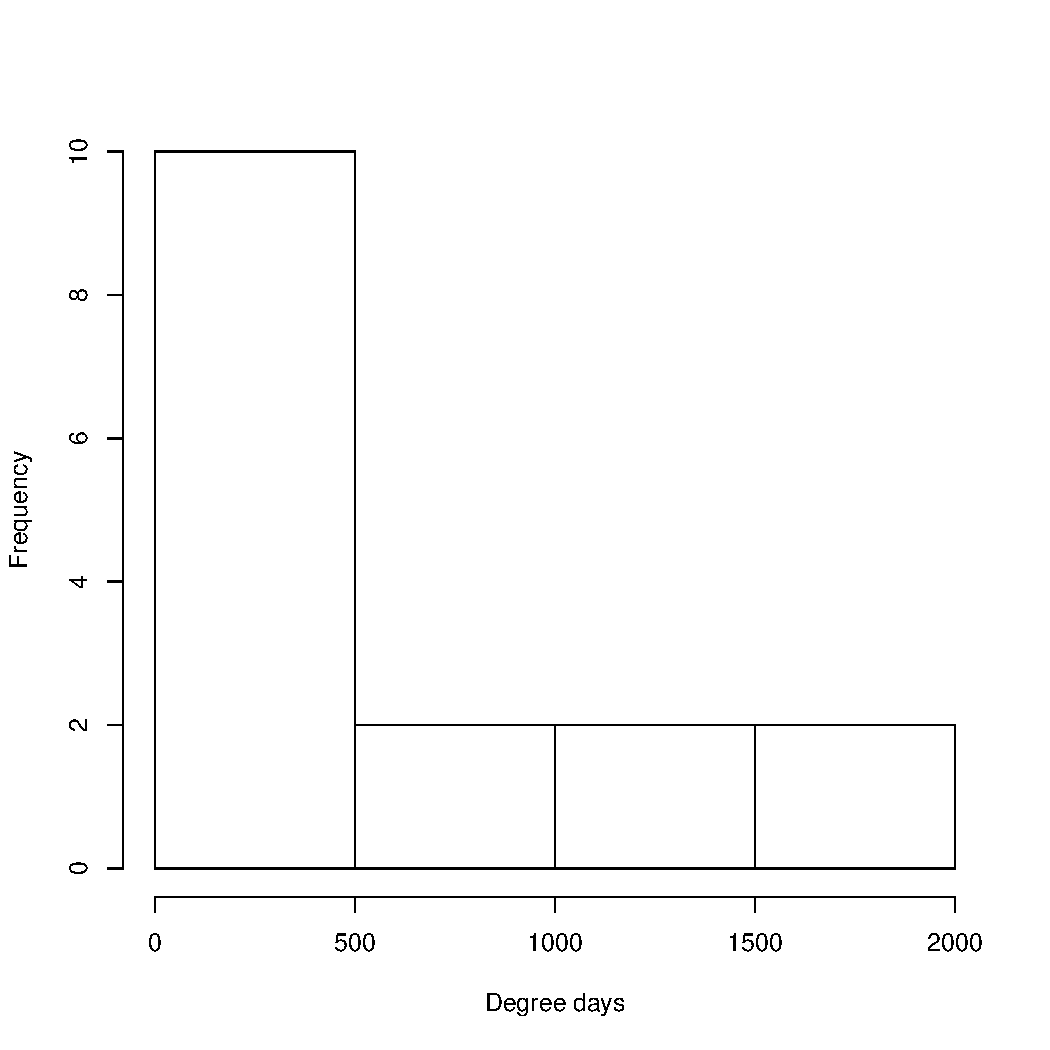
\includegraphics[width=2.1in]{degdays_all_time_steps_hist}
  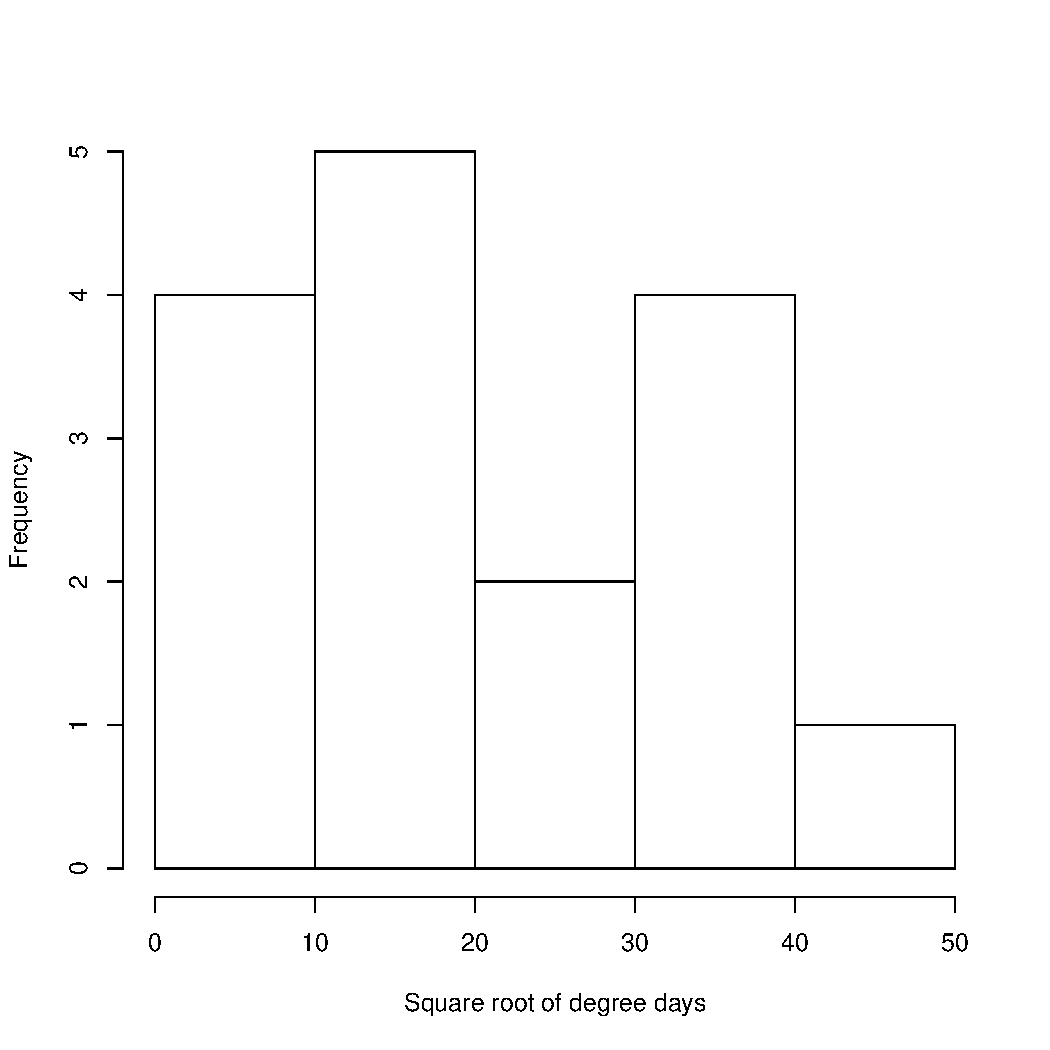
\includegraphics[width=2.1in]{sqrt_degdays_all_time_steps_hist}
\end{figure}
  }
  
\end{frame}



\begin{frame}{Looking at just the first 2 weeks}

  {\scriptsize
    \noindent I also fit random forest models separately for:\\
    - the whole range of time steps (61 days)\\
    - just the first 15 days

    \vspace{0.05in}
    
    \noindent After the first 15 days, the observations occur much
    less frequently, on the order of about once a week, so there is a
    natural breaking point in the data here.
    
\begin{figure}
  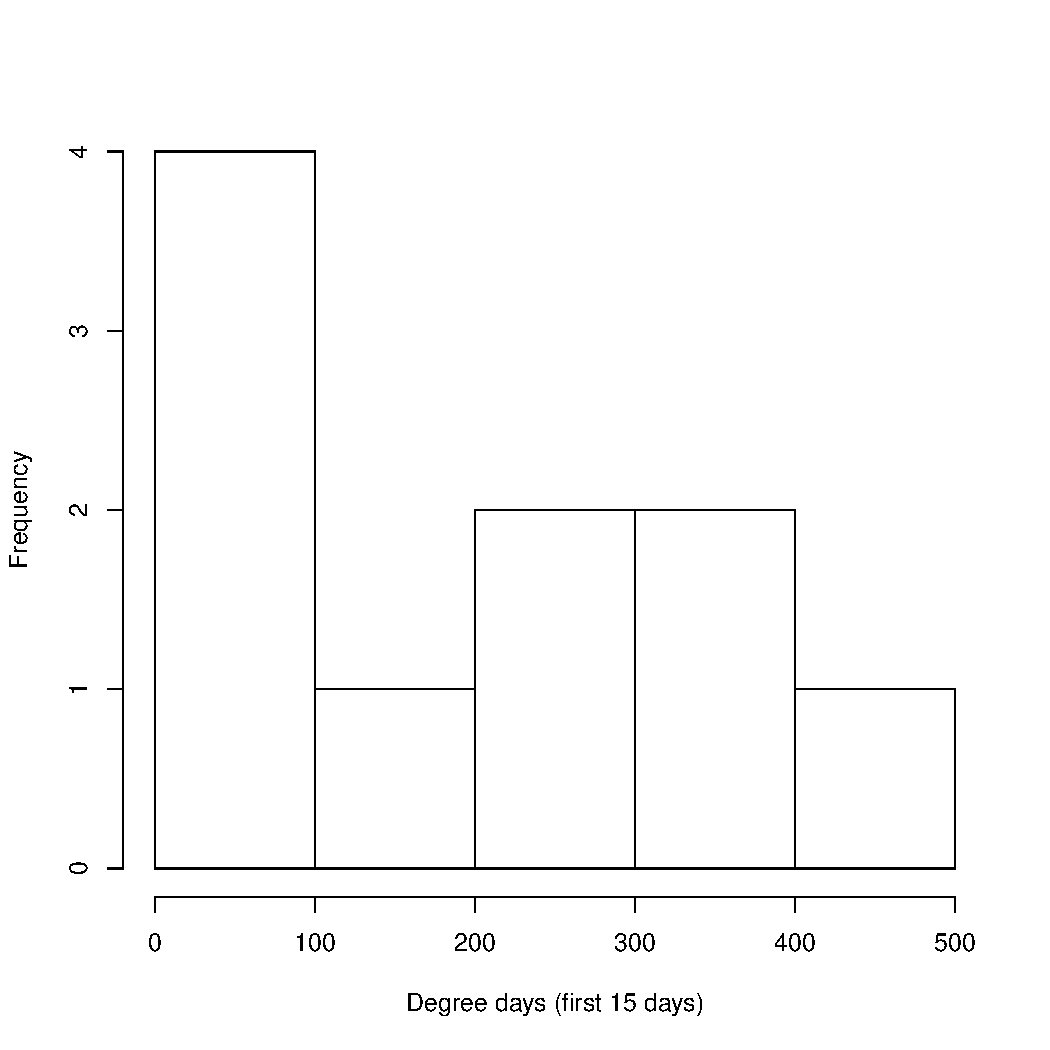
\includegraphics[width=2.1in]{degdays_first_two_weeks_hist}
  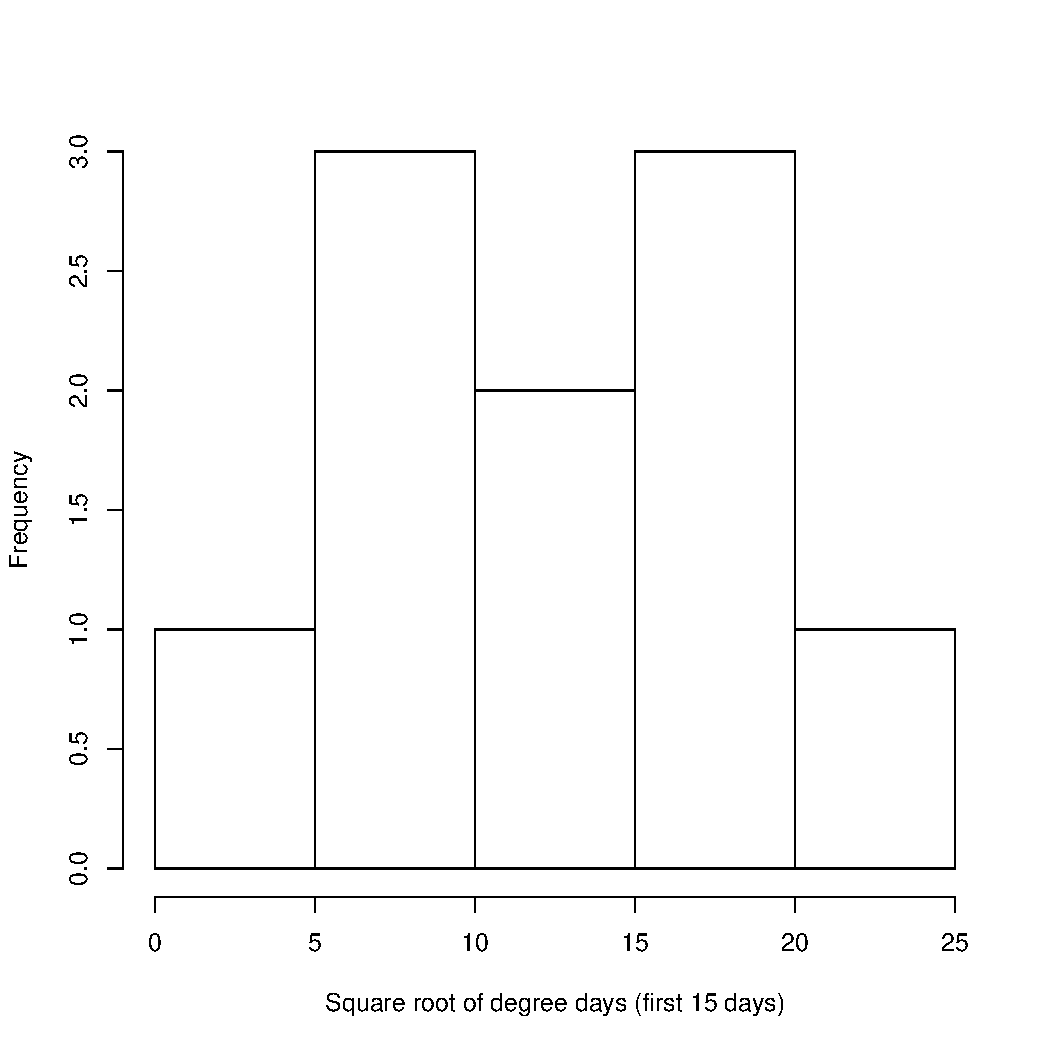
\includegraphics[width=2.1in]{sqrt_degdays_first_two_weeks_hist}
\end{figure}
  }
  
\end{frame}



\begin{frame}{Fitting the random forest models}

  {\footnotesize

    \begin{itemize}
  \item For each scenario, we have to determine the number of variables to consider for each split of the random forest decision tree.
  \item Considering only a subset of available variables at each split allows the random forest technique to work well when variables are correlated.
  \item To determine the number that works best in each scenario, we use a series of cross-validation runs, leaving out a 10\% subset of our data each time and using the remaining data to fit the model and make predictions.
    \item Each model is then fit using the number of splits that
      worked best in cross-validation runs.
      \item This was done for 16 different models.
    \end{itemize}
  }
  
\end{frame}
%% %%%%%%%%%%%%%%%%%%%%%%%%%%%%%



%% %%%%%%%%%%%%%%%%%%%%%%%%%%%%%
\section[All time steps]{Using all time steps}


\begin{frame}{Using family taxa - original units}
%% family, orig, all steps

  {\scriptsize
    
  \noindent Using original units:\\
  RMSE: 207.23  \hspace{0.05in}  Explained variation: 86.06\%

  \begin{center}
    \begin{figure}
      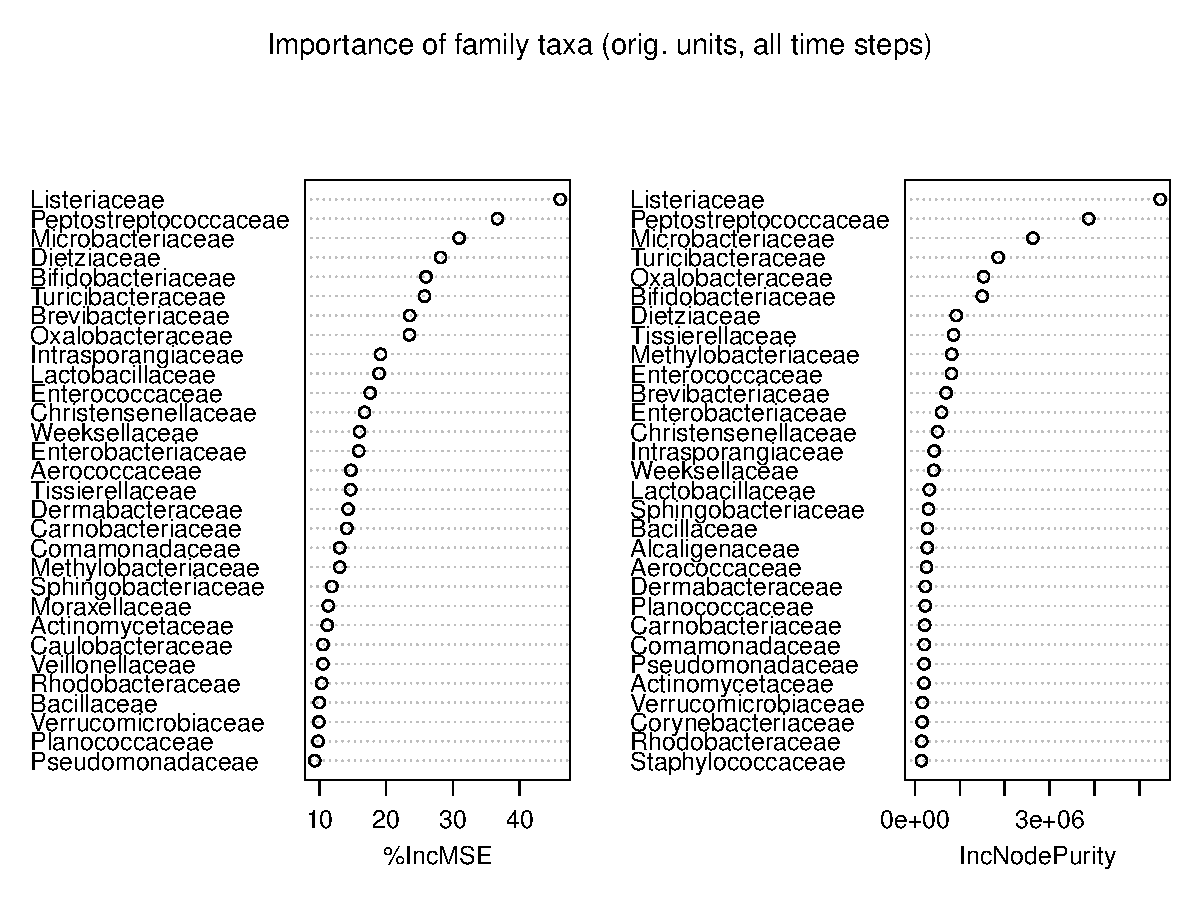
\includegraphics[width=3.25in]{../only_families/all_time_steps/orig_units_all_data_families_imp_plot}
    \end{figure}
  \end{center}
  \vspace{-0.25in}

\noindent There are 51 family-level taxa which were considered as predictors.
}

\end{frame}



\begin{frame}{Using family taxa - sqrt transformation}
  %% family, sqrt, all steps
  
  {\scriptsize
    
  \noindent Using square root transformation:\\
  RMSE: 4.41  \hspace{0.05in}  Explained variation: 87.42\%

  \vspace{0.05in}
  
  \noindent If you transform the predictions back to the original
  scale and then compare with the original degree days, the RMSE is
  approximately 226.23.
  
\begin{center}
\begin{figure}
  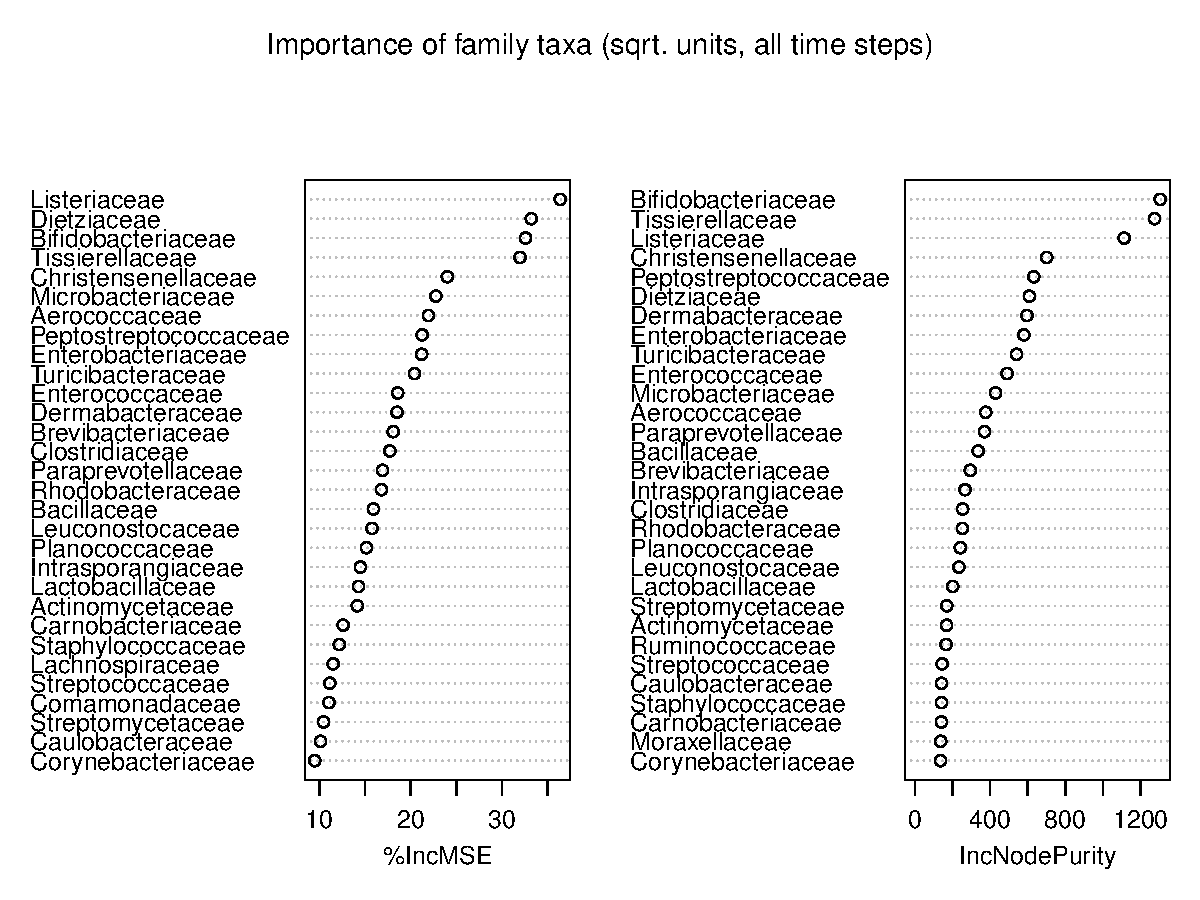
\includegraphics[width=3.25in]{../only_families/all_time_steps/sqrt_units_all_data_families_imp_plot}
\end{figure}
\end{center}
\vspace{-0.25in}
}
  
\end{frame}



\begin{frame}{Using order taxa - original units}
  %% order, orig, all steps
  
  {\scriptsize
    
  \noindent Using original units:\\
  RMSE: 236.89  \hspace{0.05in}  Explained variation: 81.79\%

  \begin{center}
    \begin{figure}
      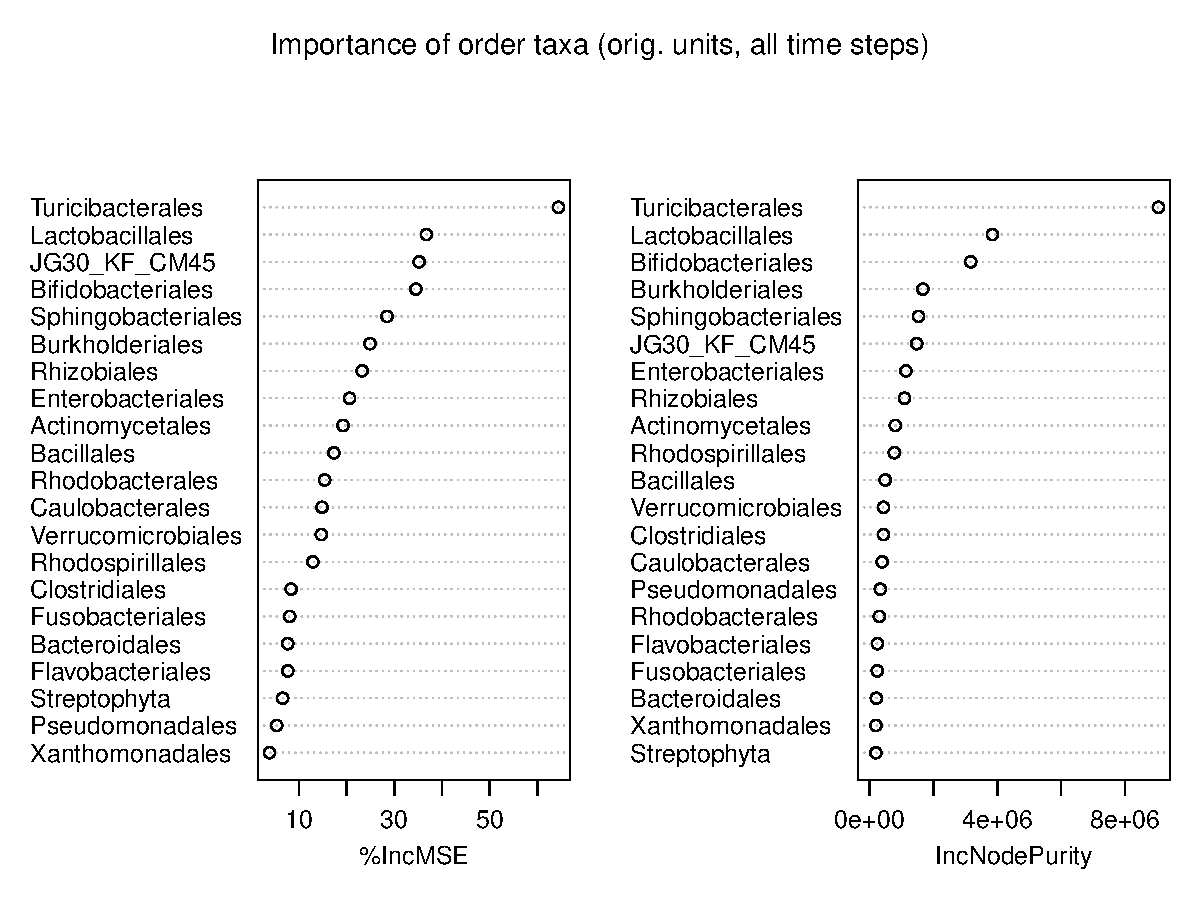
\includegraphics[width=3.25in]{../only_orders/all_time_steps/orig_units_all_data_orders_imp_plot}
    \end{figure}
  \end{center}
  \vspace{-0.25in}

\noindent There are 21 order-level taxa which were considered as predictors.
}

\end{frame}




\begin{frame}{Using order taxa - sqrt transformation}
%% order, sqrt, all steps
  
  {\scriptsize
    
  \noindent Using square root transformation:\\
  RMSE: 4.56  \hspace{0.05in}  Explained variation: 86.56\%

  \vspace{0.05in}
  
  \noindent If you transform the predictions back to the original
  scale and then compare with the original degree days, the RMSE is
  approximately 261.46.
  
\begin{center}
\begin{figure}
  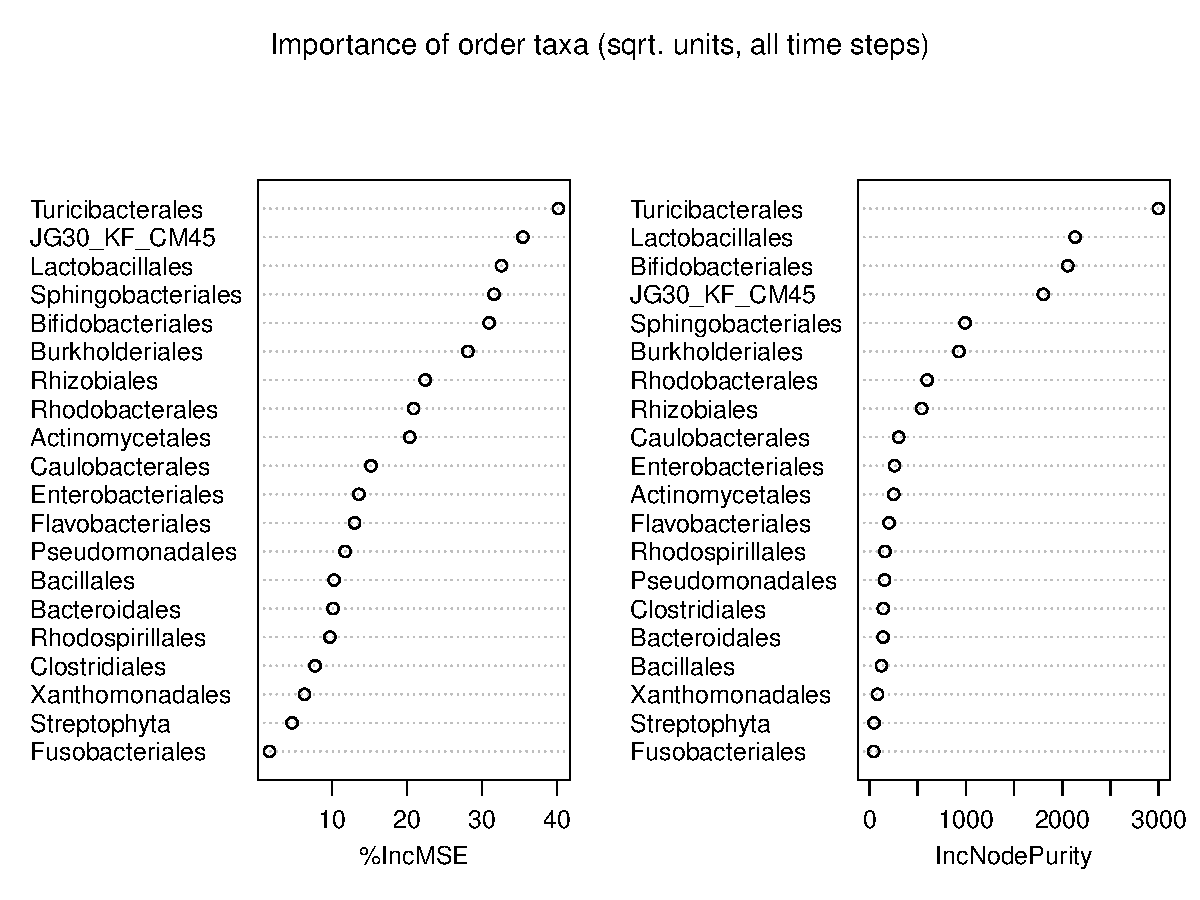
\includegraphics[width=3.25in]{../only_orders/all_time_steps/sqrt_units_all_data_orders_imp_plot}
\end{figure}
\end{center}
\vspace{-0.25in}
}
  
\end{frame}



\begin{frame}{Using combined taxa - original units}
%% combined, orig, all steps

  {\scriptsize
    
  \noindent Using original units:\\
  RMSE: 205.13  \hspace{0.05in}  Explained variation: 86.34\%

  \begin{center}
    \begin{figure}
      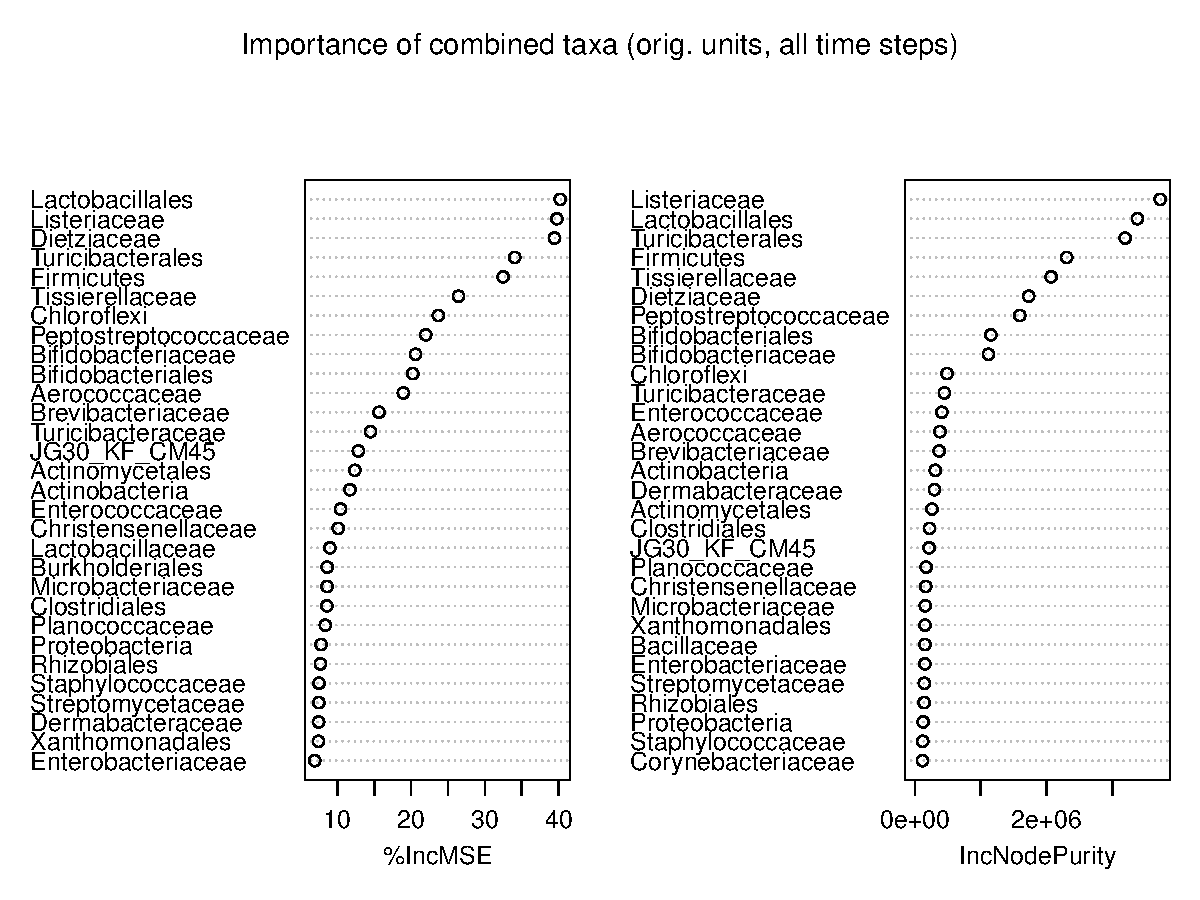
\includegraphics[width=3.25in]{../all_together/all_time_steps/orig_units_all_data_combined_imp_plot}
    \end{figure}
  \end{center}
  \vspace{-0.25in}

\noindent There are 82 taxa which were considered as predictors.
}

\end{frame}



\begin{frame}{Using combined taxa - sqrt transformation}
%% combined, sqrt, all steps
  
  {\scriptsize
    
  \noindent Using square root transformation:\\
  RMSE: 4.21  \hspace{0.05in}  Explained variation: 88.56\%

  \vspace{0.05in}
  
  \noindent If you transform the predictions back to the original
  scale and then compare with the original degree days, the RMSE is
  approximately 221.68.
  
\begin{center}
\begin{figure}
  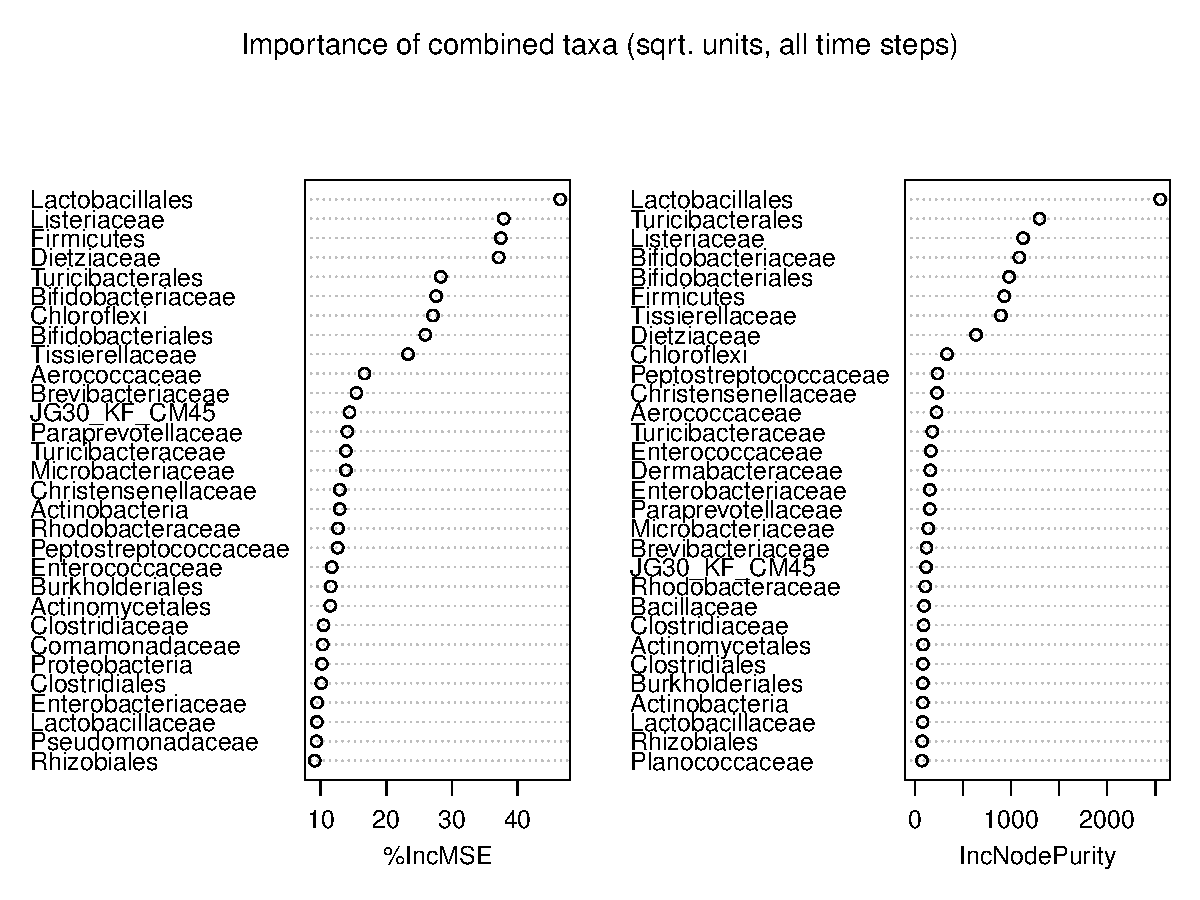
\includegraphics[width=3.25in]{../all_together/all_time_steps/sqrt_units_all_data_combined_imp_plot}
\end{figure}
\end{center}
\vspace{-0.25in}
}
  
\end{frame}




\begin{frame}{Using phylum taxa - original units}
%% phylum, orig, all steps
  
  {\scriptsize
    
  \noindent Using original units:\\
  RMSE: 313.98  \hspace{0.05in}  Explained variation: 68.01\%

  \begin{center}
    \begin{figure}
      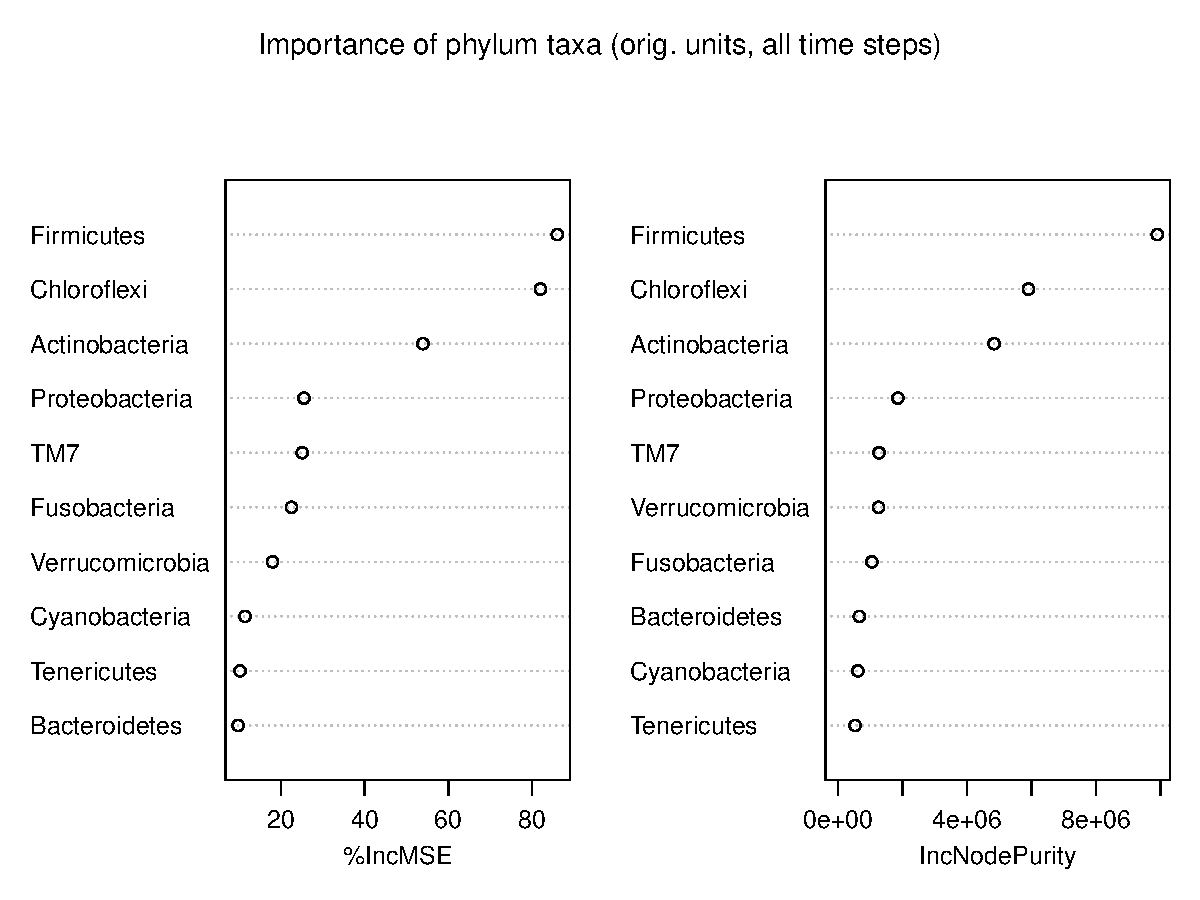
\includegraphics[width=3.25in]{../only_phyla/all_time_steps/orig_units_all_data_phyla_imp_plot}
    \end{figure}
  \end{center}
  \vspace{-0.25in}

\noindent There are 10 taxa which were considered as predictors.
}

\end{frame}



\begin{frame}{Using phylum taxa - sqrt transformation}
%% phylum, sqrt, all steps

  {\scriptsize
    
  \noindent Using square root transformation:\\
  RMSE: 6.40  \hspace{0.05in}  Explained variation: 73.50\%

  \vspace{0.05in}
  
  \noindent If you transform the predictions back to the original
  scale and then compare with the original degree days, the RMSE is
  approximately 313.28.
  
\begin{center}
\begin{figure}
  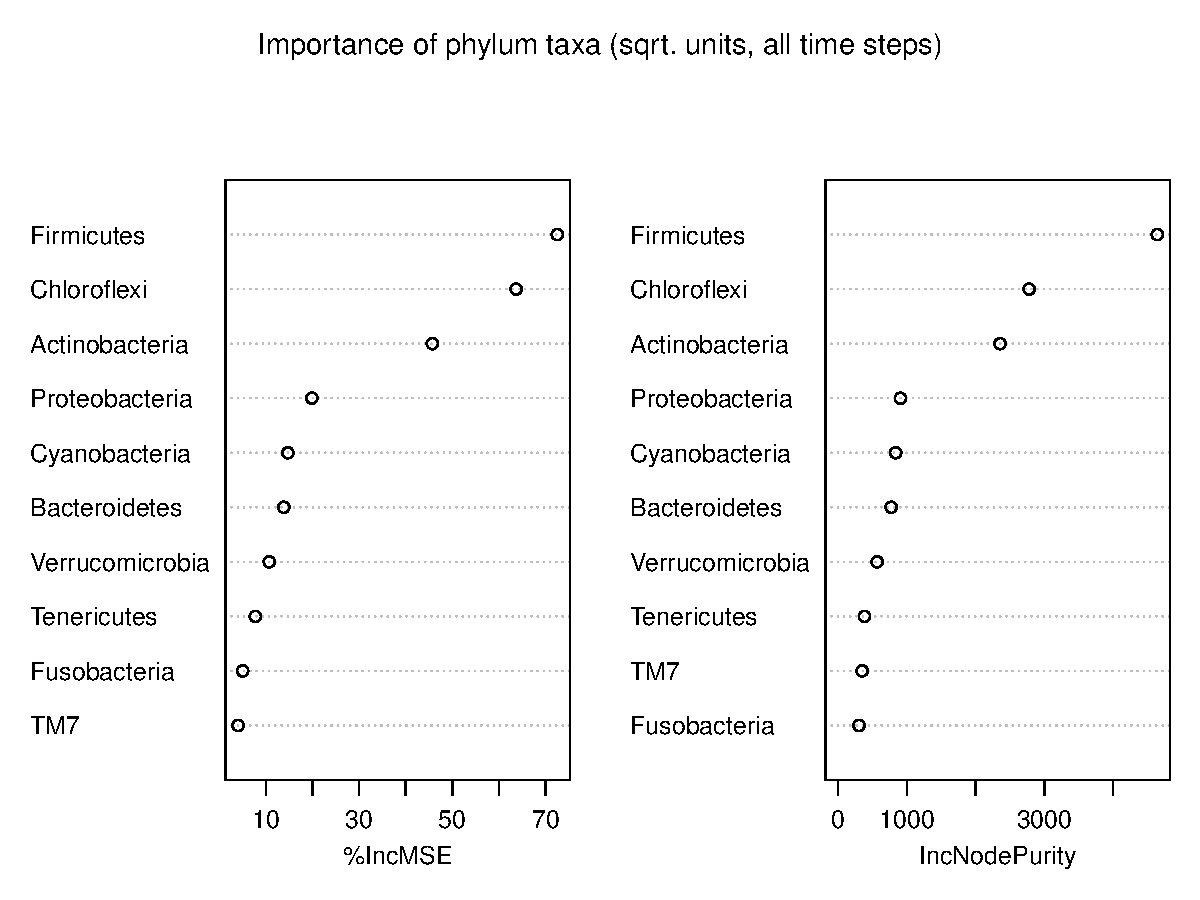
\includegraphics[width=3.25in]{../only_phyla/all_time_steps/sqrt_units_all_data_phyla_imp_plot}
\end{figure}
\end{center}
\vspace{-0.25in}
}
  
\end{frame}
%% %%%%%%%%%%%%%%%%%%%%%%%%%%%%%




%% %%%%%%%%%%%%%%%%%%%%%%%%%%%%%
\section[First 15 days]{Using first 15 days}


\begin{frame}{Using family taxa - original units}
%% family, orig, first 15
  
  {\scriptsize
    
  \noindent Using original units:\\
  RMSE: 64.29  \hspace{0.05in}  Explained variation: 82.37\%

  \begin{center}
    \begin{figure}
      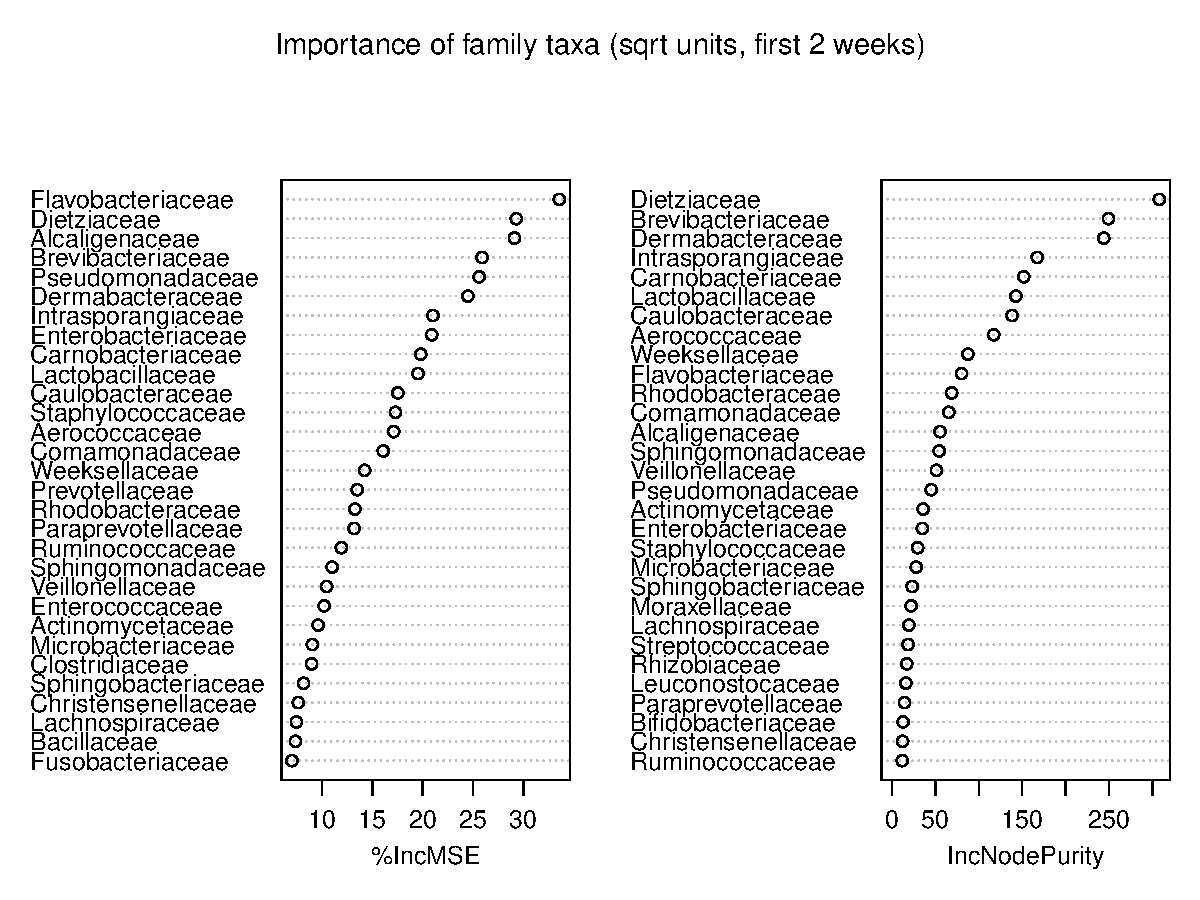
\includegraphics[width=3.25in]{../only_families/first_two_weeks/sqrt_units_first_two_weeks_families_imp_plot}
    \end{figure}
  \end{center}
  \vspace{-0.25in}

\noindent Remember, there are 51 family-level taxa which were
considered as predictors.
}

\end{frame}



\begin{frame}{Using family taxa - sqrt transformation}
%% family, sqrt, first 15

  {\scriptsize
    
  \noindent Using square root transformation:\\
  RMSE: 2.34  \hspace{0.05in}  Explained variation: 87.52\%

  \vspace{0.05in}
  
  \noindent If you transform the predictions back to the original
  scale and then compare with the original degree days, the RMSE is
  approximately 64.92.
  
\begin{center}
\begin{figure}
  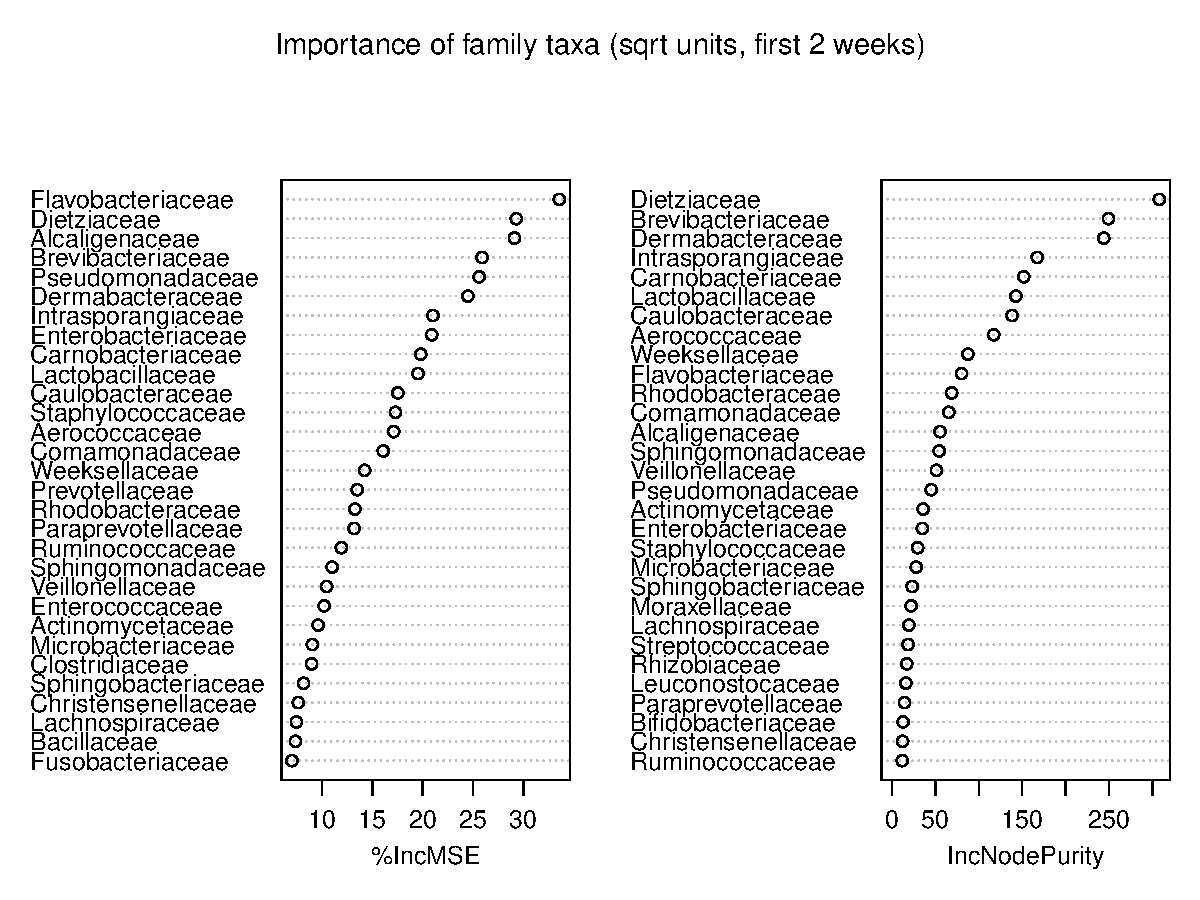
\includegraphics[width=3.25in]{../only_families/first_two_weeks/sqrt_units_first_two_weeks_families_imp_plot}
\end{figure}
\end{center}
\vspace{-0.25in}
}
  
\end{frame}



\begin{frame}{Using order taxa - original units}
%% order, orig, first 15

  {\scriptsize
    
  \noindent Using original units:\\
  RMSE: 54.38  \hspace{0.05in}  Explained variation: 87.38\%

  \begin{center}
    \begin{figure}
      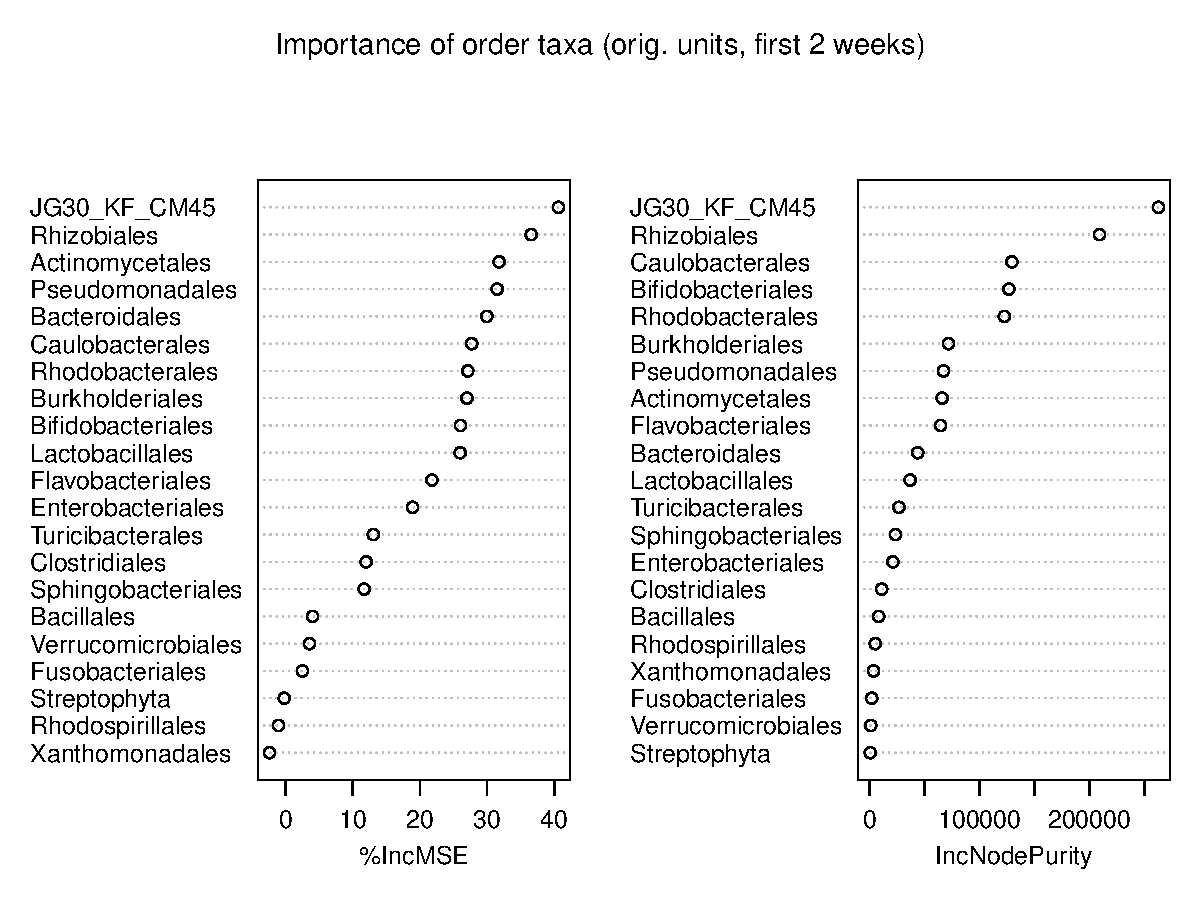
\includegraphics[width=3.25in]{../only_orders/first_two_weeks/orig_units_first_two_weeks_orders_imp_plot}
    \end{figure}
  \end{center}
  \vspace{-0.25in}

\noindent Remember, there are 21 order-level taxa which were considered as predictors.
}

\end{frame}



\begin{frame}{Using order taxa - sqrt transformation}
%% order, sqrt, first 15

  {\scriptsize
    
  \noindent Using square root transformation:\\
  RMSE: 2.08  \hspace{0.05in}  Explained variation: 90.18\%

  \vspace{0.05in}
  
  \noindent If you transform the predictions back to the original
  scale and then compare with the original degree days, the RMSE is
  approximately 52.86.
  
\begin{center}
\begin{figure}
  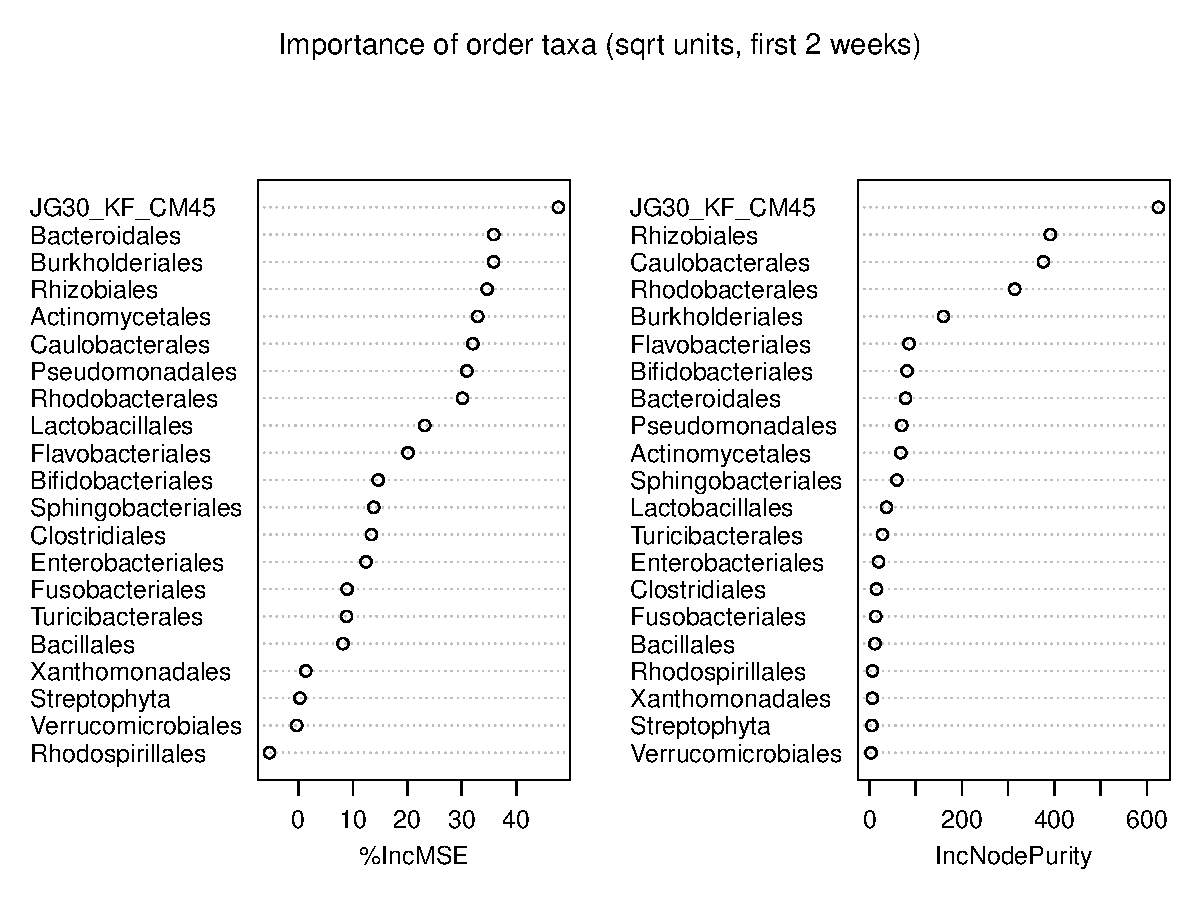
\includegraphics[width=3.25in]{../only_orders/first_two_weeks/sqrt_units_first_two_weeks_orders_imp_plot}
\end{figure}
\end{center}
\vspace{-0.25in}
}
  
\end{frame}



\begin{frame}{Using combined taxa - original units}
%% combined, orig, first 15

  {\scriptsize
    
  \noindent Using original units:\\
  RMSE: 56.95  \hspace{0.05in}  Explained variation: 86.16\%

  \begin{center}
    \begin{figure}
      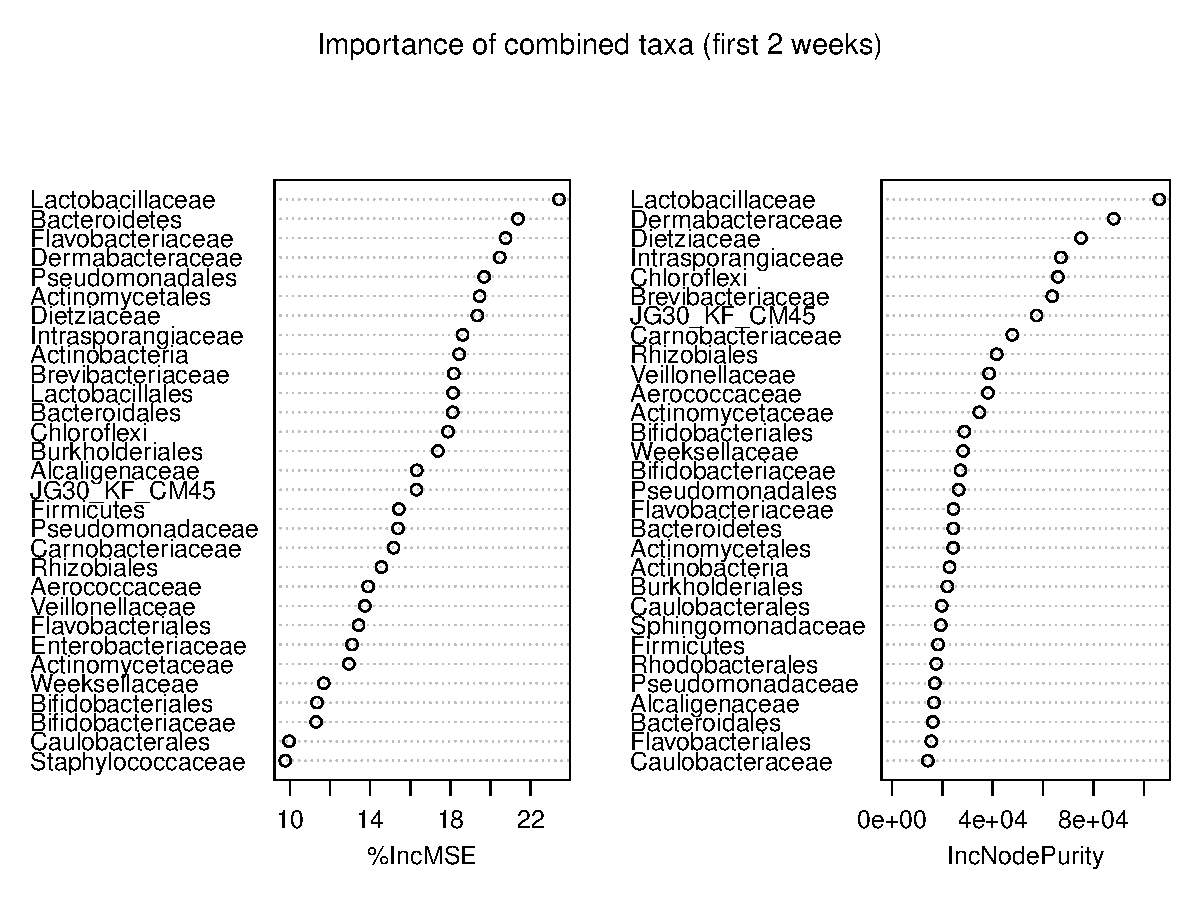
\includegraphics[width=3.25in]{../all_together/first_two_weeks/orig_units_first_two_weeks_combined_imp_plot}
    \end{figure}
  \end{center}
  \vspace{-0.25in}

\noindent Remember, there are 82 taxa which were considered as predictors.
}

\end{frame}



\begin{frame}{Using combined taxa - sqrt transformation}
%% combined, sqrt, first 15
  
  {\scriptsize
    
  \noindent Using square root transformation:\\
  RMSE: 2.14  \hspace{0.05in}  Explained variation: 89.62\%

  \vspace{0.05in}
  
  \noindent If you transform the predictions back to the original
  scale and then compare with the original degree days, the RMSE is
  approximately 56.68.
  
\begin{center}
\begin{figure}
  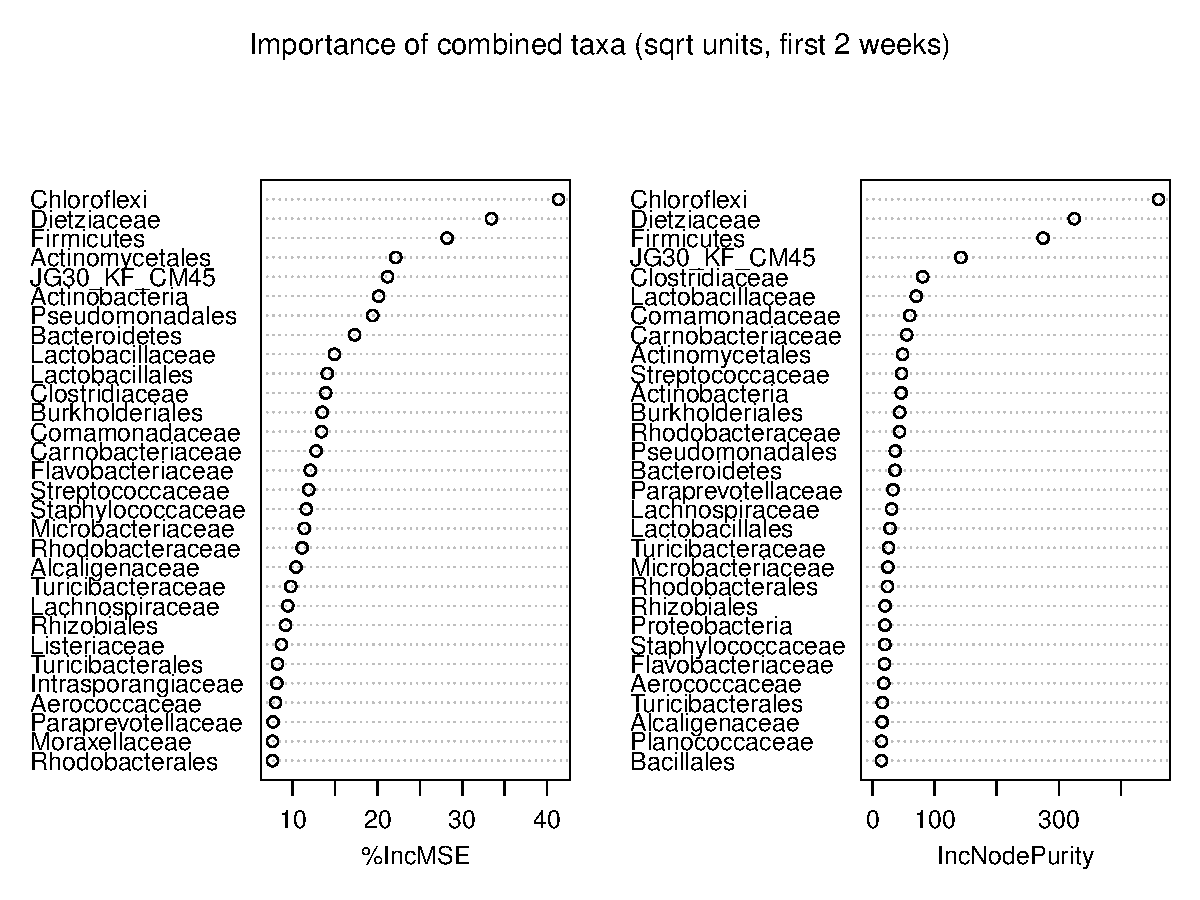
\includegraphics[width=3.25in]{../all_together/first_two_weeks/sqrt_units_first_two_weeks_combined_imp_plot}
\end{figure}
\end{center}
\vspace{-0.25in}
}
  
\end{frame}



\begin{frame}{Using phylum taxa - original units}
%% phylum, orig, first 15

  {\scriptsize
    
  \noindent Using original units:\\
  RMSE: 62.57  \hspace{0.05in}  Explained variation: 83.30\%

  \begin{center}
    \begin{figure}
      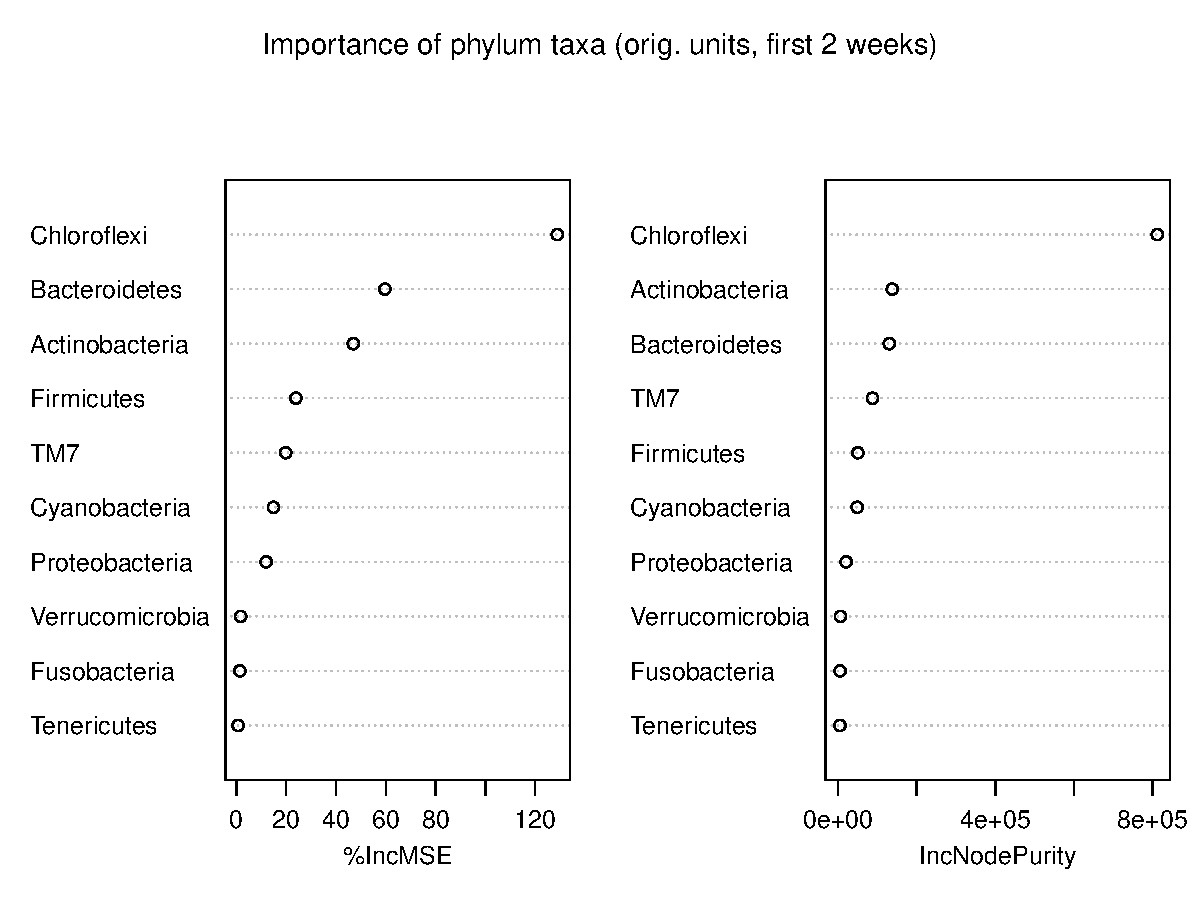
\includegraphics[width=3.25in]{../only_phyla/first_two_weeks/orig_units_first_two_weeks_phyla_imp_plot}
    \end{figure}
  \end{center}
  \vspace{-0.25in}

\noindent Remember, there are 10 taxa which were considered as predictors.
}

\end{frame}



\begin{frame}{Using phylum taxa - sqrt transformation}
%% phylum, sqrt, first 15
  
  {\scriptsize
    
  \noindent Using square root transformation:\\
  RMSE: 2.33 \hspace{0.05in}  Explained variation: 87.65\%

  \vspace{0.05in}
  
  \noindent If you transform the predictions back to the original
  scale and then compare with the original degree days, the RMSE is
  approximately 62.67.
  
\begin{center}
\begin{figure}
  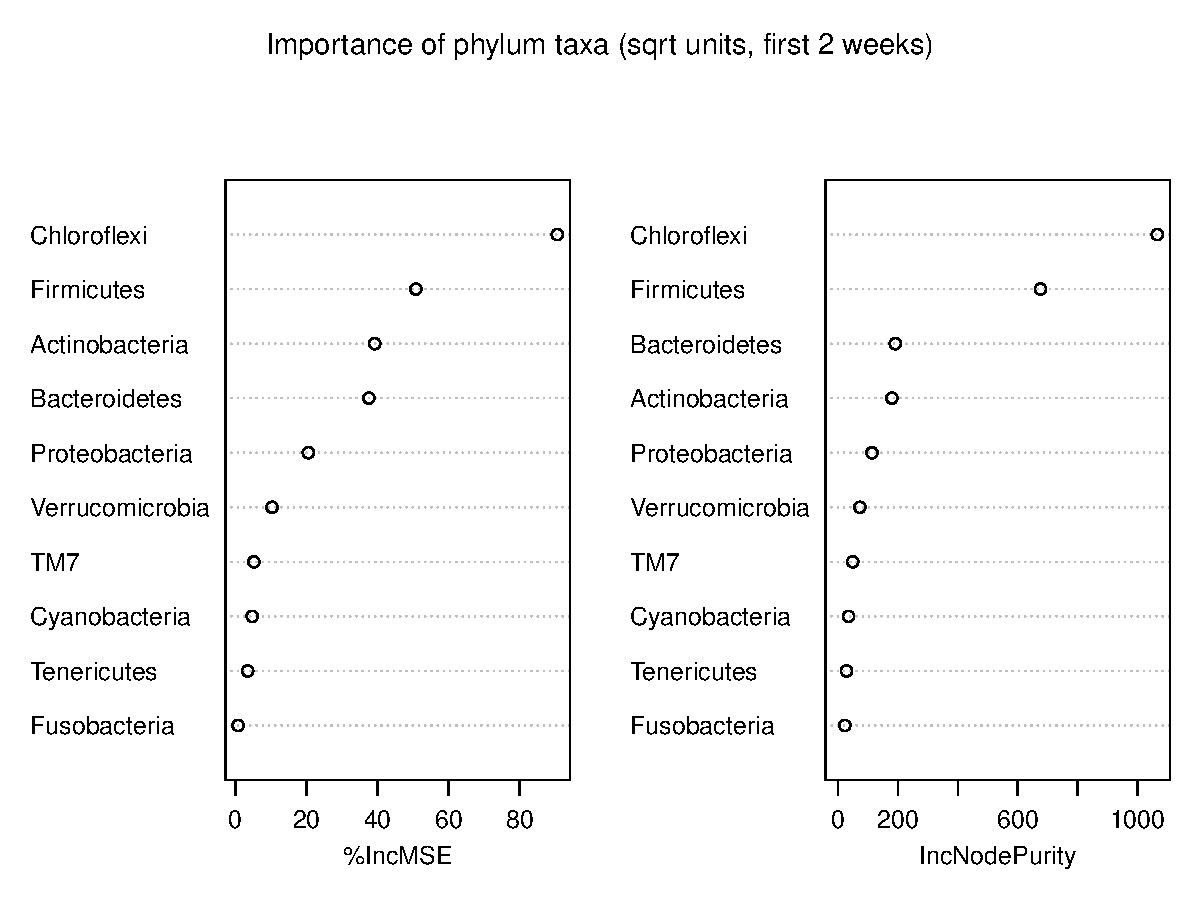
\includegraphics[width=3.25in]{../only_phyla/first_two_weeks/sqrt_units_first_two_weeks_phyla_imp_plot}
\end{figure}
\end{center}
\vspace{-0.25in}
}
  
\end{frame}
%% %%%%%%%%%%%%%%%%%%%%%%%%%%%%%





%% %%%%%%%%%%%%%%%%%%%%%%%%%%%%%
\section{Some summaries}

\begin{frame}{Best fit using all time steps, orig.~units}
  
  \noindent When using all time steps and original scale, the best fit came from using all taxa combined.


  \begin{center}
    \begin{figure}
      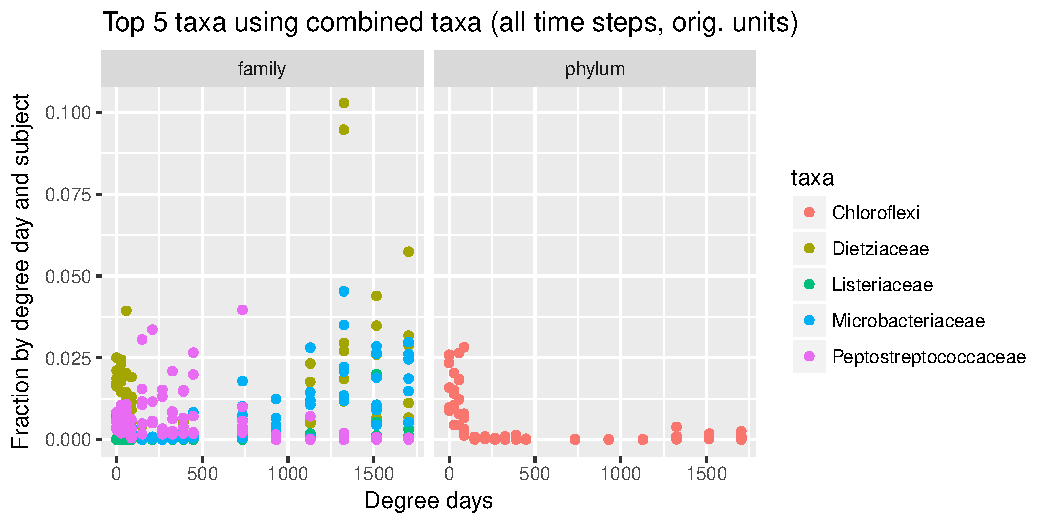
\includegraphics[width=4.5in]{combined_orig_units_all_data_top_5_taxa}
    \end{figure}
  \end{center}
  \vspace{-0.25in}
  
\end{frame}



\begin{frame}{Best fit using all time steps, sqrt.~units}

  \noindent When using all time steps and sqrt scale, the best fit also came from using all taxa combined.
  
  \begin{center}
    \begin{figure}
      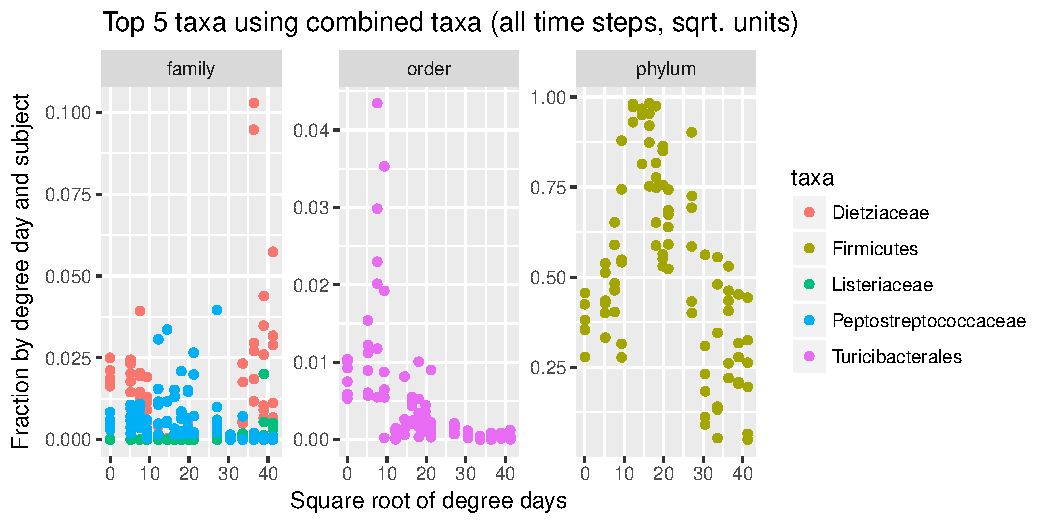
\includegraphics[width=4.5in]{combined_sqrt_units_all_data_top_5_taxa}
    \end{figure}
  \end{center}
  \vspace{-0.25in}

\end{frame}



\begin{frame}{Best fit using first 15 days, orig.~units}
  
  \noindent When using just the first 15 days on the original scale,
  the best fit came from using order taxa.

  \begin{center}
    \begin{figure}
      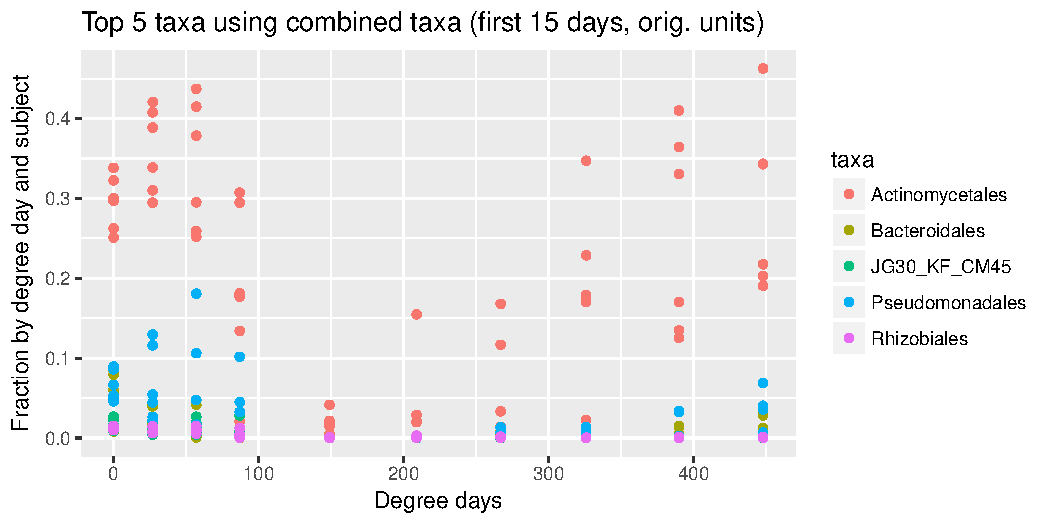
\includegraphics[width=4.5in]{orders_orig_units_first_two_weeks_top_5_taxa}
    \end{figure}
  \end{center}
  \vspace{-0.25in}
  
\end{frame}



\begin{frame}{Best fit using first 15 days, sqrt.~units}
  
  \noindent When using just the first 15 days on the sqrt.~scale,
  the best fit also came from using order taxa.

  \begin{center}
    \begin{figure}
      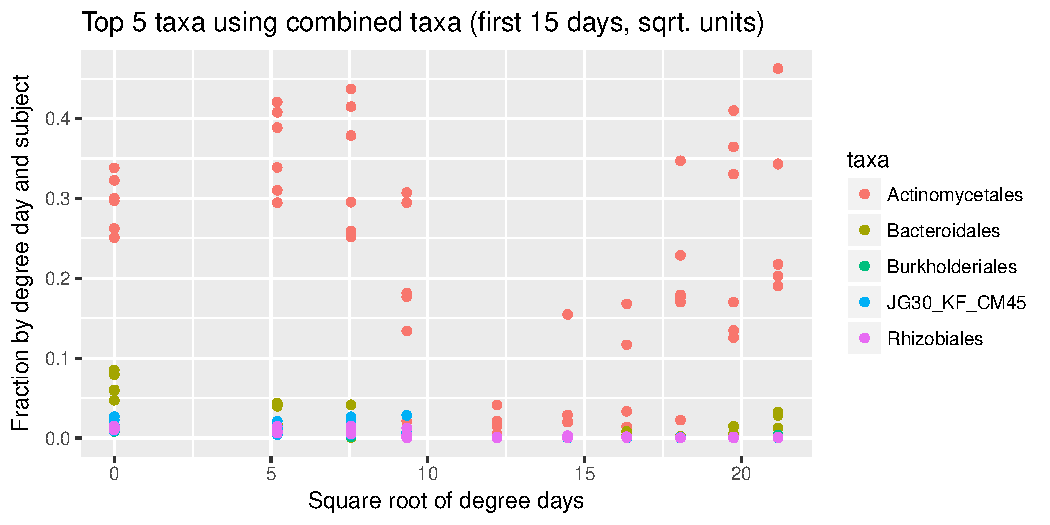
\includegraphics[width=4.5in]{orders_sqrt_units_first_two_weeks_top_5_taxa}
    \end{figure}
  \end{center}
  \vspace{-0.25in}
  
\end{frame}

%% %%%%%%%%%%%%%%%%%%%%%%%%%%%%%



\end{document}
